Στο παρόν κεφάλαιο γίνεται μια εξερεύνηση στους αλγορίθμους επιβλεπόμενης μάθησης. Αυτό επιτεύχθηκε με τη χρήση γραμμικών και μη γραμμικών ταξινομητών, διερευνώντας διαφορετικά δεδομένα εισόδου για κάθε περίπτωση. Η βιβλιοθήκη που χρησιμοποιήθηκε για τη γραμμική ταξινόμηση ονομάζεται \en{LIBLINEAR} και χαρακτηρίζεται από εξαιρετικές επιδόσεις σε προβλήματα με μεγάλα σετ δεδομένων. Αντίστοιχα, για τη μη γραμμική ταξινόμηση χρησιμοποιήθηκε η βιβλιοθήκη \en{LIBSVM}, η οποία αναγάγει τα δεδομένα εισόδου σε μεγαλύτερο χώρο διαστάσεων.
\section{Θεωρία γραμμικής ταξινόμησης}
Η βιβλιοθήκη \en{LIBLINEAR} υποστηρίζει δύο δημοφιλείς δυαδικά γραμμικούς ταξινομητές: τη λογιστική παλινδρόμηση (\en{Logistic Regression}) και τη γραμμική μηχανή υποστήριξης διανυσμάτων (\en{linear SVM}). Δεδομένου ενός σετ εκπαίδευσης $(\mathbf{x}_i, y_i)$, $i=1,...,l$, όπου $\mathbf{x}_i\in\R^n$ είναι ένα χαρακτηριστικό διάνυσμα και $y_i=\pm1$ είναι οι ετικέτες, ένας γραμμικός ταξινομητής βρίσκει ένα διάνυσμα βαρών $\mathbf{w}\in\R^n$ επιλύοντας το ακόλουθο πρόβλημα:
\begin{center}
$min_{\mathbf{w}}f(\mathbf{w})\equiv\frac{1}{2}\mathbf{w}^T\mathbf{w}+C\sum_{i=1}^{l}\xi(y_i\mathbf{w}^T x_i)$
\end{center}
όπου $\mathbf{w}^T\mathbf{w}/2$ είναι ο όρος ομαλοποίησης, $\xi(y_i\mathbf{w}^T x_i)$ είναι η συνάρτηση κόστους (\en{loss function}) και $C>0$ είναι η παράμετρος ομαλοποίησης. Θεωρούμε τις συναρτήσεις κόστους στη λογιστική παλινδρόμηση (\en{LR}), στο  \en{L1-SVM}, στο \en{L2-SVM}:
\begin{center}
$\xi_{LR}(y\mathbf{w}^T\mathbf{x})=log(1 + exp(-y\mathbf{w}^T\mathbf{x}))$\\
$\xi_{L1}(y\mathbf{w}^T\mathbf{x})=(max(0, 1 - y\mathbf{w}^T\mathbf{x}))$\\
$\xi_{L2}(y\mathbf{w}^T\mathbf{x})=(max(0, 1 - y\mathbf{w}^T\mathbf{x}))^2$
\end{center}
Σε μερικές περιπτώσεις, η συνάρτηση διακρίσεως του ταξινομητή περιλαμβάνει και έναν παράγοντα βάρους $b$. Η \en{LIBLINEAR} χειρίζεται αυτόν τον παράγοντα αυξάνοντας το διάνυσμα $\mathbf{w}$ και κάθε παράδειγμα $\mathbf{x}_i$ με μία επιπλέον διάσταση: $\mathbf{w}^T \leftarrow [\mathbf{w}^T, b]$, $\mathbf{x}_i^T \leftarrow [\mathbf{x}_i^T, B]$, όπου B είναι μια σταθερά που ορίζεται από τον χρήστη. Η προσέγγιση για το \en{L1-SVM} και το  \en{L2-SVM} είναι μέσω της μεθόδου \en{coordinate descent}. Για το \en{LR} και το \en{L2-SVM}, η \en{LIBLINEAR} υλοποιεί μια μέθοδο περιοχής εμπιστοσύνης \en{Newton}. Στη φάση των δοκιμών, εκτιμάται ένα μέλος των δεδομένων $\mathbf{x}$ σαν θετικό εάν $\mathbf{w}^T\mathbf{x}>0$, και αρνητικό σε αντίθετη περίπτωση \cite{liblinearguide}, \cite{liblinearreport}.\par
Η μηχανή διανυσμάτων υποστήριξης εντάσσεται στο γενικότερο πλαίσιο της βελτιστοποίησης κυρτών συναρτήσεων και η προσέγγισή της έχει νόημα για όλους τους γραμμικούς ταξινομητές. Σε αδρές γραμμές, η διαδικασία εξελίσσεται σε τέσσερα κύρια βήματα:
\begin{enumerate}
\item Το πρόβλημα της εύρεσης του βελτίστου υπερεπιπέδου ξεκινά με μια δήλωση του προβλήματος στον πρωτεύοντα χώρο βαρών, ως ένα πρόβλημα βελτιστοποίησης με περιορισμούς.
\item Κατασκευάζεται η συνάρτηση \en{Lagrange} του προβλήματος.
\item Διατυπώνονται οι συνθήκες για τη βελτιστοποίηση της μηχανής.
\item Στήνεται το σκηνικό για την επίλυση του προβλήματος βελτιστοποίησης στο δυικό χώρο των πολλαπλασιαστών \en{Lagrange}.
\end{enumerate}
\par Όπως προαναφέρθηκε, το πρωτεύον πρόβλημα ασχολείται με μια κυρτή συνάρτηση κόστους και γραμμικούς περιορισμούς. Δοθέντος ενός τέτοιου προβλήματος βελτιστοποίησης με περιορισμούς, είναι δυνατό να κατασκευάσουμε ένα άλλο πρόβλημα, το αποκαλούμενο δυικό του πρωτεύοντος. Αυτό το δεύτερο πρόβλημα έχει την ίδια βέλτιστη τιμή με το πρωτεύον, αλλά με τους πολλαπλασιαστές \en{Lagrange} να παρέχουν τη βέλτιστη λύση \cite{haykin}.
\section{Εξερεύνηση γραμμικών ταξινομητών}
Αρχικά έγινε μια εξερεύνηση των μεθόδων που παρέχει η \en{LIBLINEAR} για την επίλυση του προβλήματος. Λαμβάνοντας υπόψη 2.000 καταναλώσεις πελατών με ωριαίες μετρήσεις, επιλέχθηκε 10\% ποσοστό ρευματοκλοπών για την προσομοίωση. Η βιβλιοθήκη που χρησιμοποιήθηκε περιλαμβάνει 7 διαφορετικούς συνδυασμούς ταξινομητών και συναρτήσεων κόστους, για να μπορούν να αντιμετωπιστούν όσο το δυνατόν περισσότερα προβλήματα. Παρ' όλα, αυτά οι μέθοδοι \en{L1} είναι παλαιότερες εκδόσεις των \en{L2} και αναμένεται να έχουν χειρότερα αποτελέσματα στις δοκιμές. Για την σφαιρική αντιμετώπιση του προβλήματος χρησιμοποιήθηκαν όλοι οι ταξινομητές που παρέχονται από τη βιβλιοθήκη σε κάθε τύπο απάτης. Παρακάτω παρατίθενται οι συνδυασμοί ταξινομητών και συναρτήσεων κόστους που δοκιμάστηκαν και τα αποτελέσματα σε κάθε τύπο απάτης.\par
\begin{enumerate}
\item \en{L2} ομαλοποιημένη λογιστική παλινδρόμηση (πρωτεύον)
\item \en{L2} oμαλοποιημένος ταξινομητής με \en{L2} συνάρτηση κόστους διανυσμάτων υποστήριξης (δυικό)
\item \en{L2} oμαλοποιημένος ταξινομητής με \en{L2} συνάρτηση κόστους διανυσμάτων υποστήριξης (πρωτεύον)
\item \en{L2} oμαλοποιημένη ταξινομητής με \en{L1} συνάρτηση κόστους διανυσμάτων υποστήριξης (δυικό)
\item Ταξινόμηση διανυσμάτων υποστήριξης από \en{Crammer} και \en{Singer}
\item \en{L1} oμαλοποιημένος ταξινομητής με \en{L2} συνάρτηση κόστους διανυσμάτων υποστήριξης
\item \en{L1} ομαλοποιημένη λογιστική παλινδρόμηση
\item \en{L2} ομαλοποιημένη λογιστική παλινδρόμηση (δυικό)
\end{enumerate}
\par Αρχικά έγινε μια δοκιμή σε 2.000 καταναλωτές με το 10\% τους να έχει εισροή μη τεχνικών απωλειών. Τα διανύσματα των καταναλωτών είχαν 8.760 χαρακτηριστικά που αντιστοιχούν στις ώρες ενός έτους. Για να ευρεθεί η συνολική απόδοση όλων των γραμμικών ταξινομητών, έγιναν δοκιμές και στους τέσσερις τύπους απάτης (1, 2, 3, μικτός) και για αυτό και τα αποτελέσματα αναμένονται σχετικά χαμηλά. Ειδικότερα θα εξαχθεί ο μέσος όρος του \en{F1 score} και του \en{Accuracy} από τη δοκιμή κάθε αλγορίθμου και στους τέσσερις τύπους απάτης.\par
Χρησιμοποιώντας 70\% του δείγματος για τις εκπαιδεύσεις κάθε ταξινομητή και 30\% για τις προβλέψεις, πραγματοποιήθηκαν τέσσερις δοκιμές σε κάθε ένα από τους οκτώ συνολικά αλγορίθμους. Τα αποτελέσματα φαίνονται παρακάτω στον Πίνακα \ref{tab:meanlinearmetrics}.
\begin{table}[ht!]
\centering
\begin{tabular}{ |c||c|c|c|c|c|c|c|c|  }
 \hline
 Αλγόριθμος & 1 & 2 & 3 & 4 & 5 & 6 & 7& 8 \\
 \hline
 \en{F1 score} & 23.92 & 31.99 & 30.19 &  28.67& 32.66 & 29.28 & 20.43 &24.04\\
 \hline
\en{Accuracy} & 91.36 & 90.41 & 90.46 &  90.56 & 90.15 & 90.37 & 91.43 & 91.35\\
\hline
\hline
  Μέσος όρος & 57.64 & 61.2 & 60.33 & 59.61 & 61.4 & 59,83 & 55.93 & 57.7\\
\hline
\end{tabular}
\caption{Μέσος όρος \en{Accuracy} των δοκιμών}
\label{tab:meanlinearmetrics}
\end{table}
\par Εύκολα παρατηρείται από τον Πίνακα \ref{tab:meanlinearmetrics} πως η επίδοση των αλγορίθμων στο \en{F1 score} είναι περιορισμένη, υποδηλώνοντας δυσκολία στην ταξινόμηση. Αυτό οφείλεται στις κακές επιδόσεις των αλγορίθμων στις απάτες τύπου δύο, τρία και μικτού. Από την άλλη πλευρά τα αποτελέσματα του \en{Accuracy} είναι υποσχόμενα, αλλά πρέπει να ληφθεί υπόψη πως λόγω του χαμηλού ποσοστού κλοπών ένας κακός αλγόριθμος θα μπορούσε να προβλέπει πάντα αρνητικά και να είχε 90\% \en{Accuracy}. Καθίσταται, λοιπόν, σαφές πως οι ταξινομητές έχουν μεγάλη δυσκολία να διαχωρίσουν τις προσομοιώσεις μη τεχικών απωλειών με μεγάλο τυχαίο παράγοντα από τις φυσιολογικές καταναλώσεις. Παρ' όλα αυτά, τα αποτελέσματα των δοκιμών στις απάτες τύπου 1 είναι ικανοποιητικά και δημιουργούν ανάγκη περαιτέρω ανάλυσης.\par
Η διαφορά της απόδοσης των γραμμικών ταξινομητών σε κάθε είδος απάτης και ειδικότερα σε σχέση με της κλοπές τύπου 1 υπήρξε ο λόγος εκκίνησης νέου κύκλου δοκιμών. Έγινε λοιπόν δοκιμή κάθε αλγορίθμου σε απάτες τύπου 1 με 10\% ποσοστό ρευματοκλοπών. Το 70\% των δεδομένων χρησιμοποιήθηκε για τις εκπαιδεύσεις των ταξινομητών και το υπόλοιπο 30\% για τις προβλέψεις των αλγορίθμων.
\begin{table}[ht!]
\centering
\begin{tabular}{ |c||c|c|c|c|c|  }
 \hline
 Αλγόριθμος & \en{DR}  & \en{FPR} & \en{Accuracy} & \en{F1 score} & \en{BDR \%} \\
 \hline
1 & 77.44 & 1.56 & 96.37 & 80.78 & 85 \\
  \hline
2 & 79.70 & 1.81 & 96.37 & 81.23 & 83 \\
  \hline
3 &78.95 & 2.22 & 95.93 & 79.25 & 80 \\
  \hline
4 & 78.95 & 2.05 & 96.07 & 79.85 & 81\\
  \hline
5 & 78.20 & 1.81 & 96.22 & 80.31 & 83\\
 \hline
6 & 77.44 & 2.14 & 95.85 & 78.63 & 80 \\
 \hline
7 & 75.94 & 1.81 & 96.00 & 78.91 & 82\\
 \hline
8 & 79.70 & 1.81 & 96.37 & 81.23 & 83\\
 \hline
\end{tabular}
\caption{Αποτελέσματα δοκιμής τύπου 1 χωρίς κανονικοποίηση}
\label{tab:exploreclassifiers1nonorm}
\end{table}

\subsection{Παρατηρήσεις}
Παρατηρώντας τους πίνακες αποτελεσμάτων εύκολα αποδεικνύεται η αρχική υπόθεση πως οι ταξινομητές και συναρτήσεις κόστους \en{L2} έχουν καλύτερη συμπεριφορά ως προς την αντιμετώπιση του προβλήματος αναγνώρισης χρονοσειρών.  Πιο συγκεκριμένα, για την τελική επιλογή του συνδυασμού μεθόδων επιλέχθηκαν δύο μετρικές για να καθορίσουν την επιλογή του καλύτερου πακέτου. Λήφθηκε υπόψη η μεταβολή της ευστοχίας (\en{Accuracy}) και παράχθηκε μέσος όρος για όλους τους τύπους. Παράλληλα, υπολογίστηκε μέσος όρος των δοκιμών με γνώμονα το καλύτερο \en{F1 score}, καθώς είναι μια αρκετά ζυγισμένη μετρική για τα προβλήματα ταξινόμησης. Βάσει, λοιπόν, του Πίνακα \ref{tab:meanlinearmetrics} την καλύτερη επίδοση έχει το πρωτεύον πρόβλημα που αποτελείται από \en{L2} oμαλοποιημένο ταξινομητή με \en{L2} συνάρτηση κόστους διανυσμάτων υποστήριξης, καθώς όπως μπορεί και να φανεί στον Πίνακα \ref{tab:accuracytypes} του Παραρτήματο,ς η μηχανή διανυσμάτων υποστήριξης \en{Crammer} και \en{Singer} έχει καλύτερη επίδοση στους τύπους 2, 3 και στον μικτό. Αλλά, στην παρούσα φάση θα ασχοληθούμε με την απάτη τύπου 1.
\section{Εξερεύνηση διαφορετικών τρόπων κανονικοποίησης}
Το σκέλος της κανονικοποίησης των δεδομένων είναι ζωτικής σημασίας για κάθε σύστημα μηχανικής μάθησης. Η κανονικοποίηση των δεδομένων υλοποιείται, μειώνοντας το εύρος των τιμών σε οποιαδήποτε σχετικά μικρό εύρος. Συνηθέστερη πετυχημένη πρακτική είναι η αναγωγή των τιμών σε εύρος [0,1] ή [-1,1] με στόχο τη βελτίωση της επίδοσης και της ταχύτητας του αλγορίθμου.\par
Επιλέγοντας λοιπόν το σύνηθες δείγμα 2.000 καταναλωτών με ωριαίες μετρήσεις έτους και 10\% ποσοστό καταναλωτών με μη τεχνικές απώλειες, οι αλγόριθμοι εκπαιδεύτηκαν με 70\% του δείγματος και η πρόβλεψη επιτεύχθηκε με 30\% για κάθε μέθοδο κανονικοποίησης.\par
Η βελτίωση της επίδοσης του αλγορίθμου επιτυγχάνεται σε μεγάλο βαθμό στη συγκεκριμένη περίπτωση από την κανονικοποίηση στο εύρος [0,1], βελτιώνοντας σε μικρό βαθμό τις μετρικές και μειώνοντας σχεδόν 10 φορές τον χρόνο εκτέλεσης της εκπαίδευσης. Στον Πίνακα \ref{tab:explorenormalization} παρατίθενται τα αποτελέσματα των βέλτιστων ταξινομητών σε κάθε είδος κανονικοποίησης.\par

\begin{table}[ht!]
\centering
\begin{tabular}{ |c|c|c|c|c|c|c|c|  }
 \hline
 Κανονικοποίηση & \en{DR}  & \en{FPR} & \en{Accuracy} & \en{F1 score} & \en{BDR \%}& χρόνος εκπαίδευσης \en{(s)} \\
 \hline
 [0,1] & 80.87 & 1.54 & 96.96 & 81.94 & 85 & 6.492741\\
  \hline
 [-1,1]& 91.67 & 21.23 & 80.15 & 49.62 & 32 & 551.264250\\
  \hline
 - &79.70 & 1.81 & 96.37 & 81.23 & 83 & 58.246916 \\
  \hline
\end{tabular}
\caption{Αποτελέσματα κανονικοποιήσεων}
\label{tab:explorenormalization}
\end{table}

\section{Εξερεύνηση χρονικής υποδιαίρεσης χρονοσειρών}
Ολοκληρώνοντας την εξερεύνηση των ταξινομητών, απαιτείται να γίνει έλεγχος στις χρονικές υποδιαιρέσεις των χρονοσειρών. Για αυτό το σκοπό έγινε δοκιμή του πιο εύστοχου ταξινομητή σε 2.000 καταναλωτές με ποσοστό ρευματοκλοπών 10\% και μόνο απάτες τύπου 1. Στη δοκιμή οι χρονοσειρές διαιρέθηκαν σε ημερήσιες, ωριαίες και ημίωρες μετρήσεις, λαμβάνοντας υπόψη όχι μόνο τις μετρικές ευστοχίας, αλλά και τον χρόνο εκτέλεσης της εκπαίδευσης κάθε ταξινομητή. Επιλέγοντας ως συνήθως 70\% των δεδομένων για εκπαίδευση και το υπόλοιπο για πρόβλεψη, έγιναν δοκιμές για κάθε χρονική υποδιαίρεση.\par
Στον Πίνακα \ref{tab:timedivision} εμφανίζεται, όπως αναμενόταν πως όσο αυξάνεται η συχνότητα των μετρήσεων τόσο πιο εύστοχος γίνεται ο ταξινομητής. Ωστόσο, ο χρόνος εκτέλεσης της εκπαίδευσης φαίνεται να επηρεάζεται έντονα από διαφορετικές χρονικές υποδιαιρέσεις με την ταξινόμηση με συχνότητα λήξης ανά ημέρα να είναι σημαντικά γρηγορότερη από τις υπόλοιπες, αλλά παρουσιάζεται σχετική δυσκολία στην αναγνώριση της απάτης. 

\begin{table}[ht!]
\centering
\begin{tabular}{ |c||c|c|c|c|c|c|  }
 \hline
 Συχνότητα & \en{DR}  & \en{FPR} & \en{Accuracy} & \en{F1 score} & \en{BDR \%} & χρόνος εκπαίδευσης \en{(s)}\\
 \hline
μέρες & 81.62 & 2.55 & 95.85 & 79.86 & 78 & 0.069182\\
 \hline
ώρες & 82.88 & 2.16 & 96.22 & 82.59 & 81 & 4.152410\\
  \hline
ημίωρα & 81.08 & 1.66 & 96.44 & 83.33 & 84 & 12.169304\\
  \hline
\end{tabular}
\caption{Αποτελέσματα δοκιμής χρονικής υποδιαίρεσης}
\label{tab:timedivision}
\end{table}

\section{Θεωρία Μηχανών Διανυσμάτων Υποστήριξης}
Για την ταξινόμηση με μηχανές διανυσμάτων υποστήριξης επιλέχθηκε η βιβλιοθήκη \en{LIBSVM}, η οποία προέρχεται από τους ίδιους δημιουργούς της \en{LIBLINEAR}. Σκοπός του \en{SVM} είναι η παραγωγή μοντέλων (βάσει των δεδομένων εκπαίδευσης), τα οποία προβλέπουν τα χαρακτηριστικά των δεδομένων δοκιμής βάσει μόνο των πληροφοριών που αντλούνται από τις τιμές των δεδομένων.\par
Ξεκινώντας από τα δεδομένα εκπαίδευσης έχουμε ζευγάρια παραδειγμάτων-δυαδικών χαρακτηριστικών $(\mathbf{x}_i,y_i)$,$i=1,...,l$ όπου $\mathbf{x}_i\in\R^n$ και $y\in\{1,-1\}^l$, ενώ οι μηχανές διανυσμάτων υποστήριξης \en{(SVM)} απαιτούν την λύση του παρακάτω προβλήματος βελτιστοποίησης:
\begin{center}
$min_{\mathbf{w},\mathbf{b},\mathbf{\xi}} \frac{1}{2}\mathbf{w}^T\mathbf{w}+C\sum_{i=1}^l\xi_i$\\
δεδομένου $y_i(\mathbf{w}^T\phi(\mathbf{x}_i)+b)\geq 1-\xi_i$,\\
$\xi_i \geq 0$
\end{center}
\par Εδώ τα διανύσματα εκπαίδευσης $\mathbf{x}_i$ ανάγονται σε μεγαλύτερο (ίσως άπειρο) χώρο διαστάσεων από τη συνάρτηση $\phi$. Τα \en{SVM} βρίσκουν ένα γραμμικά διαχωρίσιμο υπερεπίπεδο με μέγιστο περιθώριο σε αυτό χώρο ανώτερων διαστάσεων. $C>0$ είναι ο παράγοντας που θέτει ποινή στον παράγοντα λάθους (\en{error term}). Επιπροσθέτως, η σχέση $K(\mathbf{x}_i,\mathbf{x}_j)\equiv \phi(\mathbf{x}_i)^T\phi(\mathbf{x}_j)$ ονομάζεται συνάρτηση πυρήνα. Παρόλο που νέοι πυρήνες προτείνονται από ερευνητές, έχουν θεσπιστεί οι ακόλουθοι:
\begin{itemize}
\item Γραμμικός: $K(\mathbf{x}_i,\mathbf{x}_j)= \mathbf{x}_i^T\mathbf{x}_j$.
\item Πολυωνυμικός: $K(\mathbf{x}_i,\mathbf{x}_j)= (\gamma\mathbf{x}_i^T\mathbf{x}_j+r)^d$, $\gamma=\frac{1}{2\sigma^2}>0$.
\item \en{RBF}: $K(\mathbf{x}_i,\mathbf{x}_j)= exp(-\gamma\|\mathbf{x}_i-\mathbf{x}_j\|^2)$, $\gamma>0$.
\item Σιγμοειδής: $K(\mathbf{x}_i,\mathbf{x}_j)= tanh(\gamma\mathbf{x}_i^T\mathbf{x}_j +r)$.
\end{itemize}
Εδώ τα $\gamma$, $r$ και $d$ είναι παράμετροι των πυρήνων \cite{libsvmguide}.\par
Χρησιμοποιώντας τη μέθοδο των πολλαπλασιαστών \en{Lagrange} μπορεί να διατυπωθεί το δυικό πρόβλημα για τα μη διαχωρίσιμα πρότυπα. Δοθέντος του δείγματος εκπαίδευσης $\{(\mathbf{x}_i,y_i)\}_{i=1}^N$, βρίσκονται οι πολλαπλασιαστές \en{Lagrange} $\{\alpha\}_{i=1}^N$ που μεγιστοποιούν την αντικειμενική συνάρτηση:\\
\begin{center}
$Q(\alpha)=\sum_{i=1}^N\alpha_i-\frac{1}{2}\sum_{i=1}^N\sum_{j=1}^N\alpha_i\alpha_jy_iy_j\mathbf{x}_i^T\mathbf{x}_j$
υπό τους περιορισμούς
$\sum_{i=1}^N\alpha_i d_i=0$\\
$0 \leq \alpha_i \leq C$ για $i=1,2, ...,N$\\
\end{center}
όπου $C$ είναι μια καθοριζόμενη από το χρήστη θετική παράμετρος \cite{haykin}.
\subsection{Θεωρία επιλογής πυρήνα \en{RBF}}
Γενικώς, ο πυρήνας δικτύου ακτινικής συνάρτησης βάσης (\en{RBF}) είναι μια λογική πρώτη επιλογή. Αυτός ο πυρήνας ανάγει μη γραμμικά τα δείγματα σε υψηλότερο χώρο διαστάσεων που μπορεί να διαχειριστεί την περίπτωση κατά την οποία η σχέση μεταξύ της τάξης και της τιμής είναι μη γραμμική. Επιπροσθέτως, ο γραμμικός πυρήνας είναι μια ειδική περίπτωση του \en{RBF}, καθώς ο γραμμικός πυρήνας με την παράμετρο ποινής $\check{C}$ έχει την ίδια επίδοση με τον \en{RBF} με δύο παραμέτρους ($C$,$\gamma$). Ακόμη, ο πυρήνας με σιγμοειδή συνάρτηση συμπεριφέρεται όπως με \en{RBF} για συγκεκριμένες παραμέτρους.\par
Ο δεύτερος λόγος είναι ο αριθμός των υπερπαραμέτρων, οι οποίες επηρεάζουν την πολυπλοκότητα της επιλογής μοντέλου. Ο πολυωνυμικός πυρήνας έχει περισσότερες υπερπαραμέτρους από τον \en{RBF} πυρήνα.\par
Τέλος, ο πυρήνας \en{RBF} έχει λιγότερες αριθμητικές δυσκολίες. Το χαρακτηριστικό κλειδί είναι πως το $0<K_{ij}\leq1$ είναι σταθερά του πολυωνυμικού πυρήνα του οποίου οι τιμές μπορούν να φτάνουν το άπειρο $(\gamma\mathbf{x}_i^T\mathbf{x}_j+r>1)$ ή το μηδέν $(\gamma\mathbf{x}_i^T\mathbf{x}_j+r<1)$ ενώ ο βαθμός είναι ήδη μεγάλος. Επίσης, πρέπει να σημειωθεί πως ο σιγμοειδής πυρήνας δεν είναι εφικτός με κάποιες παραμέτρους.\par
Υπάρχουν κάποιες περιπτώσεις όπου ο πυρήνας \en{RBF} δεν είναι κατάλληλος. Πιο συγκεκριμένα, όταν ο αριθμός των χαρακτηριστικών είναι πολύ μεγάλος, κάποιος θα μπορούσε να χρησιμοποιήσει τον γραμμικό πυρήνα \cite{libsvmguide}.
\section{Δοκιμή ταξινόμησης με Μηχανές Διανυσμάτων Υποστήριξης}
Η προτεινόμενη διαδικασία που ακολουθείται από τους δημιουργούς του \en{LIBSVM} είναι η εξής:
\begin{itemize}
\item Μετατροπή των δεδομένων σε αναγνωρίσιμη μορφή με το πακέτο \en{SVM}.
\item Κανονικοποίηση δεδομένων.
\item Εξέταση του \en{RBF} πυρήνα.
\item Χρήση \en{cross-validation} για την εύρεση των βέλτιστων παραμέτρων $C$ και $\gamma$.
\item Χρήση των βέλτιστων παραμέτρων $C$ και $\gamma$ για την εκπαίδευση των δεδομένων εκπαίδευσης.
\item Δοκιμή.
\end{itemize}
Έχοντας τη διαδικασία αυτή υπόψη δοκιμάστηκαν επιτυχώς δύο διαφορετικά σενάρια ταξινόμησης. Στο πρώτο σενάριο ταξινομήθηκαν οι χρονοσειρές κάθε καταναλωτή βάσει της ετήσιας κατανάλωσης του και αναγνωρίζοντας κάθε τύπο κλοπής. Στο δεύτερο σενάριο χρησιμοποιήθηκε ο πυρήνας \en{RBF} και έγινε μια προσέγγιση στην αναγνώριση των ημερήσιων μη τεχνικών απωλειών ταξινομώντας σε πρώτη φάση τις ημέρες όλων των καταναλωτών και σε δεύτερη φάση κάθε καταναλωτή \cite{libsvmguide}.
\subsection{Δοκιμή χρονοσειρών χωρίς πυρήνα}
Δεδομένης της ευστοχίας των γραμμικών ταξινομητών, θεωρήθηκε αναγκαία η δοκιμή του γραμμικού πυρήνα \en{SVM}. Παρ' όλα αυτά, η διαίσθηση δεν ήταν η μόνη κινητήριος δύναμη για την υλοποίηση αυτής της δοκιμής. Γενικότερα, αν ο αριθμός των μετρήσεων είναι μεγάλος, δεν απαιτείται να αναχθούν τα δεδομένα σε χώρο ανώτερων διαστάσεων \cite{libsvmguide}. Πρακτικά, αυτό σημαίνει πως η μη γραμμική αναγωγή δεν βελτιώνει την επίδοση του συστήματος. Ενώ είναι γενικώς αποδεκτό ότι ο πυρήνας \en{RBF} είναι τουλάχιστον καλύτερος από το γραμμικό, αυτή η δήλωση είναι αληθής, μόνο αφού έχουν επιλεχθεί οι παράμετροι ($C$,$\gamma$). Ένας γενικός κανόνας χρήσης του γραμμικού πυρήνα είναι η χρήση του όταν ο αριθμός των παραδειγμάτων (καταναλωτών) είναι μικρότερος ή σχετικός με τον αριθμό των χαρακτηριστικών (ωριαίες μετρήσεις έτους).
\subsubsection{Αποτελέσματα δοκιμής}
Η δοκιμή έγινε σε 4.500 καταναλωτές με 8.760 χαρακτηριστικά, ελέγχοντας αρχικά την επίδοση του συστήματος σε κάθε τύπο απάτης με ποσοστό ρευματοκλοπής 10\%. Το 70\% του δείγματος καταναλωτών χρησιμοποιήθηκε για την εκπαίδευση των ταξινομητών και το 30\% για τις προβλέψεις τους. Οι αλγόριθμοι του \en{LIBSVM} αναμένεται να αντιμετωπίσουν δυσκολίες στους τύπους απάτης 2, 3 και μικτό όπως και οι υπόλοιποι γραμμικοί ταξινομητές.\par 
Στον Πίνακα \ref{tab:linearSVMtypes} φαίνονται τα αποτελέσματα της δοκιμής. Γίνεται, λοιπόν, σαφές πως ο ταξινομητής μπορεί να αναγνωρίσει με αξιοπιστία μόνο τις απάτες τύπου 1, όπως και οι αντίστοιχοι ταξινομητές της \en{LIBLINEAR}. Ωστόσο, ακόμα και στα χαμηλότερα αποτελέσματα έχουμε ικανοποιητικό \en{Accuracy}, γεγονός που φανερώνει ότι ο ταξινομητής λειτουργεί όπως αναμενόταν.\par
\begin{table}[ht!]
\centering
\begin{tabular}{|c||c|c|c|c|c|c|}
\hline
Τύπος & \en{DR}  & \en{FPR} & \en{Accuracy} & \en{F1 score} & \en{BDR \%} & χρόνος εκτέλεσης (\en{s})\\
\hline
1 & 81.43 & 1.24 & 96.96 & 84.76 & 88 & 10.188667\\ 
\hline
2 & 22.63 & 7.25 & 85.63 & 24.22 & 26 & 39.489221\\
\hline
3 & 23.78 & 10.36 & 82.67 & 22.52 & 20 & 39.648516\\
\hline
Μικτός & 27.13 & 7.37 & 86.37 & 27.56 & 29 & 36.836504\\
\hline
\end{tabular}
\caption{Αποτελέσματα Γραμμικού \en{SVM} σε όλους τους τύπους απάτης}
\label{tab:linearSVMtypes}
\end{table}

Για τη βαθύτερη κατανόηση της λειτουργίας του ταξινομητή απαιτείται η παρατήρηση της σχέσης των μετρικών με την ένταση κλοπής. Η ένταση κλοπής μαθηματικοποιείται σαν ένας παράγοντας που μπορεί να ποσοτικοποιήσει πόσο απέχουν τα αλλοιωμένα δεδομένα από τις πραγματικές μετρήσεις. Ουσιαστικά είναι ο συντελεστής υποδιαίρεσης των πραγματικών μετρήσεων.\par
Τα Σχήματα \ref{fig:linearintensityres} δείχνουν πως ο ταξινομητής ξεκινά να βελτιώνεται αφότου η ένταση αυξηθεί πάνω από 30\%, καθώς το \en{DR} αυξάνεται σχεδόν γραμμικά με την ένταση και το \en{FPR} μειώνεται σταθερά μετά από αυτό το σημείο. Εκεί που ο ταξινομητής έχει τη βέλτιστη απόδοση είναι στο εύρος [70\%-90\%], αφού η κλίση της καμπύλης σε αυτά τα σημεία είναι σημαντικά μικρότερη, γεγονός που υποδεικνύει σύγκλιση.

\begin{figure}[ht!]
\centering
\begin{subfigure}[b]{0.4\textwidth}
 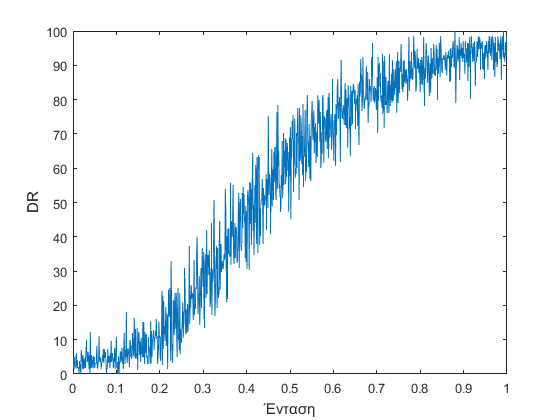
\includegraphics[width=70mm, height=50mm]{../../plots/gr_bigres_dr_intensity.png}
\caption{\en{DR} συναρτήσει της έντασης της κλοπής}
\label{fig:linearDRintensity}
\end{subfigure}
\quad
\begin{subfigure}[b]{0.4\textwidth}
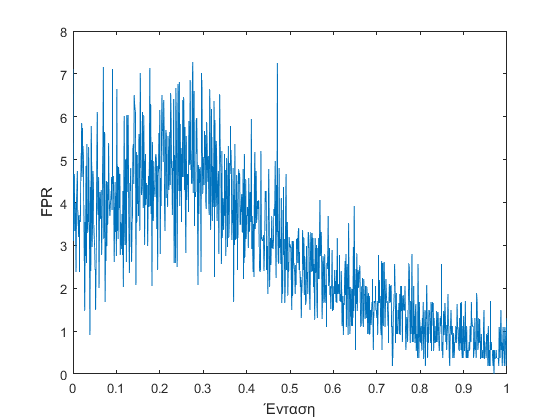
\includegraphics[width=70mm, height=50mm]{../../plots/gr_bigres_fpr_intensity.png}
\caption{\en{FPR} συναρτήσει της έντασης της κλοπής}
\label{fig:linearFPRintensity}
\end{subfigure}
\caption{Επίπτωση της έντασης στα αποτελέσματα}
\label{fig:linearintensityres}
\end{figure}
\newpage
\subsection{Ημερήσια ταξινόμηση με πυρήνα \en{RBF}}
\label{sec:RBFkernel}
Σε αυτή τη φάση δημιουργήθηκε η ανάγκη για εξαγωγή χαρακτηριστικών, ώστε να μειωθούν οι διαστάσεις των πινάκων και να επιταχυνθεί η διαδικασία. Παράλληλα, τα χαρακτηριστικά παρέχουν ένα επίπεδο αποπροσωποποίησης δημιουργώντας ένα αποτύπωμα της καταναλωτικής συνήθειας \cite{giwrgis}. Μετρώντας τα αθροίσματα, τα ελάχιστα, τα μέγιστα και τους μέσους όρους των καθημερινών καταναλώσεων δημιουργείται ένας βασικός κορμός χαρακτηριστικών για κάθε καταναλωτή που μπορεί εύκολα να επεκταθεί και σε άλλα γραμμικά και μη εξαρτώμενα χαρακτηριστικά.
\begin{itemize}
\item \textit{Μέγιστο και ώρα μεγίστου}
\item \textit{Ελάχιστο και ώρα ελαχίστου}
\item \textit{Άθροισμα κατανάλωσης ανά ημέρα}
\item \textit{Μέσος όρος, διακύμανση και τυπική απόκλιση ανά ημέρα}
\item \textit{Παράγοντας φορτίου, ελάχιστο προς μέση τιμή, ελάχιστο προς μέγιστο}
\item \textit{Επίδραση βραδινής κατανάλωσης}
\item \textit{Λοξότητα και Κύρτωση}
\end{itemize}
\par Η πρώτη δοκιμή του \en{SVM} έγινε με επιλογή 300 τυχαίων καταναλωτών μιας περιοχής με σκοπό να εκπαιδευτεί το σύστημα, ώστε να μπορεί να αναγνωρίζει ημέρες απάτης μέσα στο έτος. Η εκπαίδευση του ταξινομητή έγινε με τα ημερήσια χαρακτηριστικά για κάθε καταναλωτή. Τα δεδομένα διαχωρίζονται σε 2 τμήματα, το τμήμα της εκπαίδευσης που περιέχει 70\% του δείγματος των καταναλωτών και το τμήμα της δοκιμής που περιέχει ένα ποσοστό της τάξης του 30\% από το ίδιο δείγμα.\par
Ο ταξινομητής, λοιπόν, εκπαιδεύεται με ημερήσια χαρακτηριστικά κάθε καταναλωτή, αλλά θα πρέπει να αποφανθεί στο τέλος αν ο καταναλωτής έχει νοθεύσει τις μετρήσεις του ή όχι. Η λύση δόθηκε εισάγοντας ένα όριο ημερών το οποίο, αν ο ταξινιμητής το προσπερνούσε, τότε ο καταναλωτής θεωρείται πως έχει αλλοιώσει τα δεδομένα του. Για να βρούμε την βέλτιστη τιμή αυτού του ορίου, χρησιμοποιήθηκαν \en{ROC} καμπύλες για να παρατηρηθεί η μεταβολή του \en{DR} και \en{FPR}, ενώ αλλάζει το όριο ημερών.\\
\subsubsection{Αποτελέσματα δοκιμής}
Ελέγχοντας τα αποτελέσματα του Πίνακα \ref{tab:ROC50data}, παρατηρείται πως επιλέγοντας όριο στις 10 ημέρες επιτυγχάνεται ακρίβεια της τάξης του 95\% στην εύρεση της απάτης, αλλά με σχετικά υψηλό ποσοστό λάθος συναγερμού της τάξης του 15\% για τις έντονες απάτες. Αν χρειαστεί να ελαχιστοποιηθεί το \en{FPR}, θα πρέπει να επιλεχθεί μια μεγαλύτερη οριακή τιμή όπως το 14, που έχει ικανοποιητικό ποσοστό και στο \en{DR} που είναι της τάξης του 85\% και στο \en{FPR} που είναι της τάξης του 8\%. Οι απάτες που έγιναν με μικρότερη ένταση δεν γίνονται αντιληπτές από τον ταξινομητή που παράγει καμπύλη με παρόμοια κλίση με αυτή της ευθείας αναφοράς $y=x$.\par
Αντίστοιχα, στον Πίνακα \ref{tab:ROC35data} φαίνεται πως η μείωση του ποσοστού απάτης (\en{FR}) επηρέασε το σύστημα, και ειδικότερα μείωσε το όριο στις 10 μέρες με \en{DR}=85\% και \en{FPR}=9\%. Ουσιαστικά φαίνεται πως το σύστημα χρειάζεται και άλλους καταναλωτές, ώστε να αποτυπωθούν και οι καμπύλες για χαμηλότερες εντάσεις διείσδυσης στα δεδομένα. 

\begin{figure}[ht!]
\centering
\includegraphics[width=140mm, height=100mm]{../../plots/ROC50_1.png}
\caption{Καμπύλη \en{ROC} για \en{FR}=0.50 \label{fig:ROC50}}
\end{figure}

\begin{table}[ht!]
\begin{center}
\begin{tabular}{ |c|c|c|c|c|  }
 \hline
 \multicolumn{5}{|c|}{\en{300 IDs, 0.5 rate, 0-100 threshold}} \\
 \hline
 Όριο (Μέρες)    & \en{DR} (0.8) & \en{FPR} (0.8) & \en{DR} (0.5) & \en{FPR} (0.5) \\
 \hline
2 &	 97,917 &	40,385 &	76,712 &	35,0649\\
4 &	 97,143 &	25,625 & 	65,972 &	22,436\\
6 &	 95,683 &	22,360 &	54,225 &	13,924\\
8 &	 95,588 &	16,463 &	45,588 &	6,098\\
10 & 96,241 &	13,772 &	37,879 &	3,571\\
12 & 90,698 &	10,526 &	31,783 &	1,17\\
14 & 86,614 &	8,671  &	26,190 &	1,149\\
16 & 84,8	&	5,714  &	19,355 &	0\\
18 & 82,787 &	6,18   &	15,702 &	0\\
20 & 79,832 &	5,525  &	11,667 &	0\\
\hline
\end{tabular}
\end{center}
\caption{Πίνακας επιλογής ορίου \en{FR}=0.5 \label{tab:ROC50data}}
\end{table}

\begin{figure}[ht!]
\centering
\includegraphics[width=140mm, height=100mm]{../../plots/ROC35.png}
\caption{Καμπύλη \en{ROC} για \en{FR}=0.35 \label{fig:ROC35}}
\end{figure}
\clearpage
\begin{table}[ht!]
\begin{center}
\begin{tabular}{ |c|c|c| }
 \hline
 \multicolumn{3}{|c|}{\en{300 IDs, 0.35 rate, 0-100 threshold}} \\
 \hline
 Όριο (Μέρες)   & \en{DR} (0.8) & \en{FPR} (0.8)\\
 \hline
2 &	 95,192 &	30,612\\
4 &	 91,176 &	23,232\\
6 &	 89,691 &	17,734\\
8 &	 85,567 &	12,808\\
10 & 85,106 &	8,738\\
12 & 84,444 &	5,238\\
14 & 79,545 &	2,830\\
16 & 75		&	2,830\\
18 & 68,235 &	2,791\\
20 & 63,529 &	2,791\\
\hline
\end{tabular}
\end{center}
\caption{Πίνακας επιλογής ορίου \en{FR}=0.35 \label{tab:ROC35data}}
\end{table}

\section{Σχόλια}
Συνοψίζοντας, καθίσταται σαφές πως μπορεί να χρησιμοποιηθεί επιτυχώς επιβλεπόμενη μάθηση για τον εντοπισμό μη τεχνικών απωλειών. Οι γραμμικοί ταξινομητές μπορούν να αναγνωρίσουν αξιόπιστα και γρήγορα τον πρώτο τύπο απάτης, ενώ έχουν δυσκολία εντοπισμού στους υπόλοιπους τύπους. Παρ' όλα αυτά, χρησιμοποιώντας τον πυρήνα \en{RBF}, γίνεται εφικτή η αναγνώριση μη τεχνικών απωλειών αρχικά κάθε ημέρας και εν συνεχεία κάθε καταναλωτή. Γενικότερα, όμως, και οι δύο ομάδες ταξινομητών έχουν καλές επιδόσεις στον εντοπισμό ρευματοκλοπών με έντονη ένταση κλοπής, ενώ όσο μειώνεται η ένταση οι ταξινομητές δείχνουν μεγαλύτερη δυσκολία να διαχωρίσουν αλλοιωμένα από κανονικά δεδομένα.\par
Παράλληλα, γίνεται εμφανής η ανάγκη για σωστή επιλογή της δομής των δεδομένων εισόδου, καθώς κάθε ταξινομητής απαιτεί διαφορετική μεταχείριση. Οι γραμμικοί ταξινομητές απαιτούν πολλά χαρακτηριστικά (μετρήσεις), ενώ οι μη γραμμικοί μπορούν να λειτουργήσουν με πολύ λιγότερα. Αντίστοιχα, η κανονικοποίηση προσφέρει άμεση βελτίωση στα αποτελέσματα και επιταχύνει τη διαδικασία εκπαίδευσης σε μεγάλο βαθμό.